\documentclass[12pt]{ctexart}
\usepackage[a4paper,margin=1in]{geometry}
\usepackage{booktabs}
\usepackage{graphicx}
\usepackage{amsmath}
\usepackage{float}
\usepackage{caption}
\usepackage{setspace}
\usepackage{array}
\captionsetup{font=small}
\setstretch{1.25}

\title{组织规模、人力资本结构与上市公司违规风险\\来自中国上市公司的面板证据}
\author{作者匿名}
\date{\today}

\begin{document}
\maketitle

\begin{abstract}
企业违规的形成既受到外部监管约束，也受到企业内部组织能力的影响。本文基于 2015--2022 年中国上市公司基本信息、员工结构与违规记录数据，构建公司--年份层面的非平衡面板，系统考察组织规模与人力资本结构对违规风险的影响。与仅停留于相关性描述的研究不同，本文在经验设计上依次引入行业和年份固定效应、公司固定效应、滞后解释变量以及基于 2016--2019 年预处理特征构造的准实验分组，以提高识别强度；在结果解释上进一步从行政执行网络与业务执行网络两个通道展开机制分析。研究发现：第一，员工规模与技能员工规模在行业和年份固定效应规格下均与违规概率显著负相关；第二，在公司固定效应框架下，这一结论依然成立，且滞后技能员工规模对违规概率与违规强度均表现出显著抑制作用；第三，以 2020 年后外部环境冲击为背景，高技能预暴露企业和大规模预暴露企业的违规风险下降更为明显；第四，机制结果表明，较高的人力资本投入显著伴随着更强的行政执行网络和业务执行网络扩张，而违规率下降主要与业务执行网络的强化更为一致。整体而言，本文的证据表明，企业违规风险不仅是治理约束问题，也是组织结构与执行能力问题。本文同时发现，安慰剂检验并未完全支持强平行趋势假设，因此对准实验结果的解释仍应保持审慎。本文的贡献在于，将组织经济学视角、企业违规研究与员工结构数据结合起来，为理解企业合规能力的形成机制提供了新的经验证据。
\end{abstract}

\noindent\textbf{关键词：} 企业违规；组织规模；人力资本；公司治理；机制检验；面板数据

\section{引言}
企业违规是公司金融、制度经济学与监管经济学中的核心议题。既有文献通常强调外部监管、公司治理结构、激励扭曲与代理问题在企业违规形成中的作用。然而，从组织经济学视角看，企业违规并不仅仅是外部约束失灵的结果，也可能反映企业内部执行体系、信息处理能力与制度化流程的差异。一个治理结构相似、监管环境相近的企业，若拥有更大的组织规模、更充分的人力资本积累以及更完善的执行网络，其违规风险是否会系统性下降，仍然是一个值得进一步研究的问题。

这一问题的重要性体现在两个层面。第一，在一般性意义上，企业违规研究需要从“谁来监督企业”进一步拓展到“企业内部何以能够被有效约束”。若内部组织能力本身就是影响合规水平的重要条件，则传统仅从外部治理出发的解释框架并不完整。第二，在具体性意义上，中国上市公司在样本期内经历了监管趋严、信息披露规则完善以及外部经营环境明显变化等过程，这使得企业组织结构与违规风险之间的关系更容易在面板数据中被观察到。换言之，中国上市公司样本既提供了足够丰富的制度背景，也为识别企业内部组织能力的边际作用提供了现实场景。

本文的核心研究问题是：组织规模和人力资本结构是否能够显著降低上市公司违规风险？若答案为是，那么这一影响究竟体现为一般性的组织能力提升，还是通过更具体的行政执行网络、业务执行网络等中介机制发挥作用？围绕这些问题，本文基于上市公司年度基本信息、员工结构和违规记录，构建 2015--2022 年公司--年份层面的非平衡面板，并从三个层次展开经验分析。其一，在基准层面，使用行业与年份固定效应、公司固定效应以及滞后解释变量考察结论的稳健性。其二，在识别层面，利用企业在 2016--2019 年形成的预处理技能投入和预处理规模特征，将 2020 年后外部环境变化视作共同冲击，构建类似差分中的差分的比较框架。其三，在机制层面，分别考察行政执行网络与业务执行网络是否构成重要传导通道。

本文的贡献主要体现在以下三个方面。第一，在研究视角上，本文将企业违规问题与组织经济学、人力资本和执行能力联系起来，突出“组织约束”这一被相对忽视但具有普遍性的解释维度。第二，在数据使用上，本文将员工结构长表整理为公司--年份层面的组织变量，构造出能够直接用于违规研究的组织规模、人力资本和执行网络代理变量。第三，在经验设计上，本文并不满足于简单相关性检验，而是尝试结合公司固定效应、滞后解释变量、预处理分组、机制通道和安慰剂检验，尽可能提升结果的识别含量与论文的说服力。

\section{文献背景与研究假说}
经典经济学研究早已指出，违法与违规行为具有明确的激励结构。Becker（1968）表明，违法行为取决于收益、被查处概率与惩罚强度之间的权衡。将这一逻辑放入现代企业情境，违规可以被理解为管理层和组织在成本收益约束下作出的偏离规则选择。Jensen and Meckling（1976）以及 Fama and Jensen（1983）进一步强调，在所有权与控制权分离的条件下，代理冲突、信息不对称与监督不充分会放大偏离行为发生的可能性。由此，企业违规的根本约束既包括外部监管，也包括内部治理与组织控制。

在公司治理文献中，Shleifer and Vishny（1997）强调治理安排的核心在于限制控制权滥用与利益侵占；Dyck, Morse, and Zingales（2010）则显示，企业欺诈的暴露依赖于员工、媒体、市场机构等多元主体。这些研究凸显了监督与信息流的重要性，但对于企业内部组织结构本身如何塑造合规能力，关注仍然不够充分。Baucus（1994）提出，企业违法是压力、机会与组织倾向共同作用的结果，其中“组织倾向”实际上就包含了制度化管理能力、流程严密性和执行网络等组织特征。

基于上述文献，本文将员工规模和技能员工规模视为企业组织能力的核心代理变量。组织规模更大，通常意味着更细化的职能分工、更高的流程标准化水平以及更强的内部监督基础；技能员工更多，则意味着企业在信息处理、规则理解、内部协调和合规执行方面可能具有更高能力。进一步地，组织能力未必直接作用于违规行为，而可能通过更具体的执行网络发挥作用。例如，行政岗位扩张可能提升制度落实和内部控制能力，业务岗位扩张则可能改善流程衔接、业务记录和合规执行的覆盖范围。

基于这一分析，本文提出三个可检验假说。假说 1：组织规模越大、技能员工越多，企业违规风险越低。假说 2：在外部环境冲击发生后，预处理时期组织能力更强的企业具有更低的违规风险增幅，从而表现出更好的合规韧性。假说 3：组织能力主要通过强化企业内部执行网络而非单纯技术投入发挥作用，其中业务执行网络可能是更直接的传导通道。

\section{数据、变量与经验设计}
本文的数据来自三个部分。第一，上市公司年度基本信息表提供公司代码、行业、地区、注册资本、上市日期和上市状态等企业特征。第二，上市公司人员结构表记录公司在不同岗位和学历类别下的员工人数。第三，违规事件表记录企业违规事件、处罚金额及相关公告信息。本文按照公司代码和年份对三类数据进行匹配，构建公司--年份层面的非平衡面板。

\noindent 样本共包含     31734 个公司--年份观测，违规虚拟变量均值为 0.135，违规次数均值为 0.394。员工规模对数均值为 7.402，技能员工规模对数均值为 5.879，注册资本对数均值为 20.105，上市年限均值为 11.513。
\noindent 以 2016--2019 年企业平均技能投入和平均员工规模构造预处理分组后，高技能预暴露组样本量为     15030，大规模预暴露组样本量为     15165，2020--2022 年后冲击期观测量为     14353。这些设定为后续的固定效应、准实验与机制分析提供了统一样本基础。


在变量构造方面，本文将\textbf{违规虚拟变量}作为核心被解释变量，即若企业在某一年度存在违规记录，则取值为 1，否则为 0；同时使用 $\ln(1+\text{违规次数})$ 作为违规强度的替代指标。核心解释变量包括\textbf{员工规模对数}与\textbf{技能员工规模对数}。前者用于刻画组织总体规模，后者用于刻画更高层次的人力资本投入。控制变量包括\textbf{注册资本对数}与\textbf{上市年限}。在机制分析中，本文进一步构造 \textbf{行政执行网络} 与 \textbf{业务执行网络}，分别以行政类员工对数和业务类员工对数表示。

本文的经验设计分为三层。第一层为基准规格，在行业与年份固定效应、公司固定效应和滞后解释变量框架下考察主要结论是否稳健。第二层为准实验设计。具体而言，本文根据企业在 2016--2019 年的平均技能投入和平均组织规模，将样本划分为高技能预暴露组与大规模预暴露组，再利用 2020 年后的共同环境变化构建“预处理特征 $\times$ 后冲击”的比较框架，以考察组织能力在外部冲击下的合规韧性差异。第三层为机制设计，检验技能投入与组织规模是否推动了行政执行网络和业务执行网络扩张，并考察将这些通道变量纳入主回归后，核心系数是否被部分吸收。

基准模型可写为：
\begin{equation}
Violation_{it} = \alpha + \beta_1 \ln(Employee_{it}) + \beta_2 \ln(Skill_{it}) + \gamma X_{it} + \lambda_t + \mu_i + \varepsilon_{it},
\end{equation}
其中 $\mu_i$ 表示公司固定效应，$\lambda_t$ 表示年份固定效应，$X_{it}$ 为控制变量。准实验模型则进一步引入预处理特征与后冲击交互项，用于识别不同组织能力企业在冲击前后违规表现的差异。

\section{描述性事实}
表 \ref{tab:desc} 报告了主要变量的描述统计。违规虚拟变量均值为 0.135，说明样本期内约 13.5\% 的公司--年份观测伴随违规记录。违规次数均值为 0.394，但最大值达到 38，显示违规行为在公司之间分布高度不均。员工规模对数均值为 7.402，技能员工规模对数均值为 5.879，说明样本企业在组织规模和人力资本积累方面具有较大异质性。行政执行网络和业务执行网络的均值也较高，表明绝大多数上市公司已经具有较完整的职能分工结构。

\begin{table}[H]
\centering
\caption{主要变量描述统计}
\label{tab:desc}
\begin{tabular}{lccccc}
\toprule
                    &           N&        Mean&          SD&         Min&         Max\\
\midrule
违规虚拟变量        &       31734&       0.135&       0.341&       0.000&       1.000\\
违规次数            &       31734&       0.394&       1.051&       0.000&      38.000\\
员工规模对数        &       31734&       7.402&       1.816&       0.000&      13.253\\
技能员工规模对数    &       31734&       5.879&       1.867&       0.000&      12.784\\
研发员工对数        &       31734&       5.530&       1.688&       0.000&      12.300\\
ln\_admin\_emp        &       31734&       5.528&       1.308&       0.000&      12.120\\
ln\_business\_emp     &       31734&       4.798&       1.853&       0.000&      12.840\\
注册资本对数        &       31734&      20.105&       1.249&      10.051&      30.455\\
上市年限            &       30675&      11.513&       8.303&       1.000&      33.000\\
\\
\bottomrule
\end{tabular}
\end{table}

图 \ref{fig:scatter} 展示了员工规模与平均违规率之间的非参数关系。样本按员工规模对数分为 20 组后，平均违规率总体呈现随组织规模上升而下降的趋势。虽然该图不能构成因果识别证据，但它表明负向关系并非完全由少数极端观测驱动。

\begin{figure}[H]
\centering
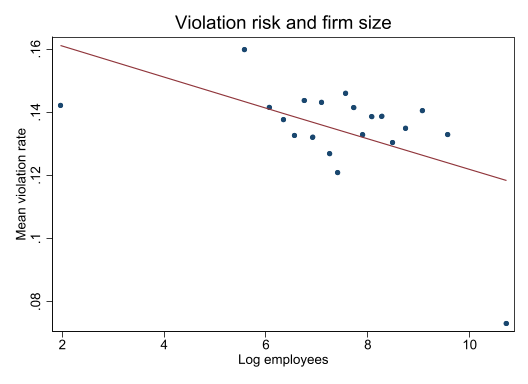
\includegraphics[width=0.70\textwidth]{../图片/paper_scatter.png}
\caption{组织规模与平均违规率}
\label{fig:scatter}
\end{figure}

图 \ref{fig:trend} 报告了样本期内平均违规率的时间变化。整体上看，违规率在 2018--2020 年处于相对高位，而后逐渐回落。与此同时，表 \ref{tab:trend} 显示技能员工规模总体持续上升，这意味着组织能力变量在时间维度上并非静止不变，而是伴随着企业成长和环境变化动态演进。

\begin{table}[H]
\centering
\caption{年度趋势统计}
\label{tab:trend}
\begin{tabular}{ccccc}
\toprule
年份 & 平均违规率 & 平均违规次数 & 平均员工规模对数 & 平均技能员工对数\\
\midrule
2015 & 0.127 & 0.306 & 7.652 & 5.637\\
2016 & 0.142 & 0.337 & 7.648 & 5.783\\
2017 & 0.119 & 0.330 & 7.341 & 5.763\\
2018 & 0.141 & 0.393 & 7.374 & 5.851\\
2019 & 0.144 & 0.467 & 7.346 & 5.917\\
2020 & 0.144 & 0.429 & 7.316 & 5.913\\
2021 & 0.135 & 0.420 & 7.440 & 5.988\\
2022 & 0.125 & 0.416 & 7.262 & 6.014\\
\bottomrule
\end{tabular}
\end{table}

\begin{figure}[H]
\centering
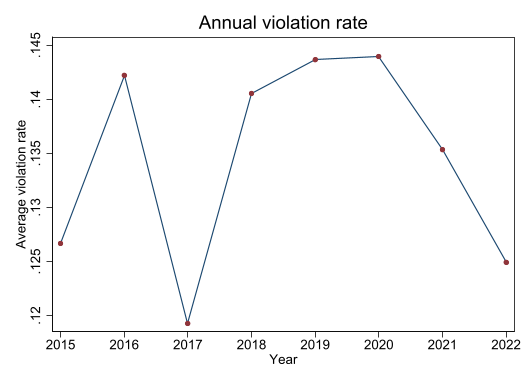
\includegraphics[width=0.70\textwidth]{../图片/paper_trend.png}
\caption{样本期内平均违规率年度变化}
\label{fig:trend}
\end{figure}

\section{基准结果与识别强化}
表 \ref{tab:main} 报告本文的主结果。第 (1) 列在行业和年份固定效应下估计，员工规模对数与技能员工规模对数的系数分别为 $-0.0195$ 和 $-0.0116$，均在 1\% 水平上显著。这表明，即使控制行业结构和宏观年份冲击，组织规模与人力资本投入较高的企业仍表现出更低的违规概率。

第 (2) 列在公司固定效应框架下重新估计。结果显示，员工规模对数与技能员工规模对数依旧显著为负，说明结论并非完全来自企业之间不随时间变化的异质性，而在企业内部的时间变化上同样成立。换言之，同一企业在组织扩张或技能投入上升的年份，其违规概率更低。

第 (3) 和第 (4) 列进一步引入滞后解释变量，以减弱反向因果和同步性偏误的担忧。结果显示，滞后技能员工规模对违规虚拟变量和违规强度均显著为负，而滞后组织规模的系数不再显著。这一结果具有重要含义：相较于简单的人员扩张，真正能够持续降低违规风险的可能是更高质量的人力资本积累。该发现使研究结论从一般性的“企业越大越少违规”，推进到更具体的“技能型人力资本是更稳健的治理性投入”。

\begin{table}[H]
\centering
\caption{主结果：组织能力与违规风险}
\label{tab:main}
\def\sym#1{\ifmmode^{#1}\else\(^{#1}\)\fi}
\begin{tabular}{l*{4}{c}}
\toprule
                    &\multicolumn{1}{c}{(1)}&\multicolumn{1}{c}{(2)}&\multicolumn{1}{c}{(3)}&\multicolumn{1}{c}{(4)}\\
\midrule
员工规模对数        &     -0.0195\sym{***}&     -0.0162\sym{***}&                     &                     \\
                    &    (0.0023)         &    (0.0057)         &                     &                     \\
\addlinespace
技能员工规模对数    &     -0.0116\sym{***}&     -0.0114\sym{***}&                     &                     \\
                    &    (0.0018)         &    (0.0032)         &                     &                     \\
\addlinespace
注册资本对数        &      0.0325\sym{***}&      0.0255\sym{***}&      0.0083         &      0.0143         \\
                    &    (0.0032)         &    (0.0063)         &    (0.0070)         &    (0.0092)         \\
\addlinespace
上市年限            &      0.0041\sym{***}&      0.0100\sym{***}&      0.0070\sym{***}&      0.0192\sym{***}\\
                    &    (0.0004)         &    (0.0014)         &    (0.0016)         &    (0.0021)         \\
\addlinespace
L1\_ln\_total\_emp     &                     &                     &      0.0004         &     -0.0093         \\
                    &                     &                     &    (0.0065)         &    (0.0088)         \\
\addlinespace
L1\_ln\_skill\_emp     &                     &                     &     -0.0092\sym{**} &     -0.0129\sym{***}\\
                    &                     &                     &    (0.0037)         &    (0.0047)         \\
\addlinespace
Constant            &     -0.3315\sym{***}&     -0.3071\sym{**} &     -0.0562         &     -0.1595         \\
                    &    (0.0694)         &    (0.1200)         &    (0.1346)         &    (0.1767)         \\
\midrule
Observations        &       30675         &       30675         &       25954         &       25954         \\
R-squared           &       0.040         &       0.008         &       0.004         &       0.010         \\
Specification       &行业+年份 FE         &     公司 FE         &公司 FE + 滞后         &    违规强度         \\
\\
\bottomrule
\end{tabular}
\end{table}

线性规格虽然便于解释，但也可能掩盖组织能力的非线性边际效应。为此，本文进一步在公司固定效应框架下加入员工规模和技能员工规模的二次项。表 \ref{tab:nonlinear} 显示，员工规模的一次项为负、二次项为正，表现出一定的 U 形特征；技能员工规模的一次项为正、二次项为负，则更接近倒 U 形关系。对违规虚拟变量而言，员工规模对数的二次项系数为 0.0034，在 5\% 水平上显著，表明组织扩张在较低到中等区间可能降低违规风险，但当组织过于庞大时，边际治理收益可能递减，甚至出现协调成本上升和层级复杂化问题。相反，技能员工规模的倒 U 形结果意味着，在较低水平技能投入阶段，企业增加技能员工可能先伴随业务复杂度提升，但当技能投入进一步增加后，其治理收益开始主导，违规风险重新下降。图 \ref{fig:ushape} 给出了员工规模非线性预测关系的直观展示。

\begin{table}[H]
\centering
\caption{非线性检验：组织规模与技能投入的 U 形关系}
\label{tab:nonlinear}
\def\sym#1{\ifmmode^{#1}\else\(^{#1}\)\fi}
\begin{tabular}{l*{2}{c}}
\toprule
                    &\multicolumn{1}{c}{(1)}&\multicolumn{1}{c}{(2)}\\
\midrule
员工规模对数        &     -0.0494\sym{***}&     -0.0494\sym{**} \\
                    &    (0.0180)         &    (0.0240)         \\
\addlinespace
ln\_total\_emp\_sq     &      0.0034\sym{**} &      0.0028         \\
                    &    (0.0015)         &    (0.0019)         \\
\addlinespace
技能员工规模对数    &      0.0243\sym{**} &      0.0504\sym{***}\\
                    &    (0.0099)         &    (0.0132)         \\
\addlinespace
ln\_skill\_emp\_sq     &     -0.0045\sym{***}&     -0.0083\sym{***}\\
                    &    (0.0011)         &    (0.0015)         \\
\addlinespace
注册资本对数        &      0.0266\sym{***}&      0.0452\sym{***}\\
                    &    (0.0064)         &    (0.0088)         \\
\addlinespace
上市年限            &      0.0107\sym{***}&      0.0218\sym{***}\\
                    &    (0.0014)         &    (0.0018)         \\
\addlinespace
Constant            &     -0.3249\sym{**} &     -0.7294\sym{***}\\
                    &    (0.1388)         &    (0.1894)         \\
\midrule
Observations        &       30675         &       30675         \\
R-squared           &       0.009         &       0.020         \\
Outcome             &违规虚拟变量         &    违规强度         \\
\\
\bottomrule
\end{tabular}
\end{table}

\begin{figure}[H]
\centering
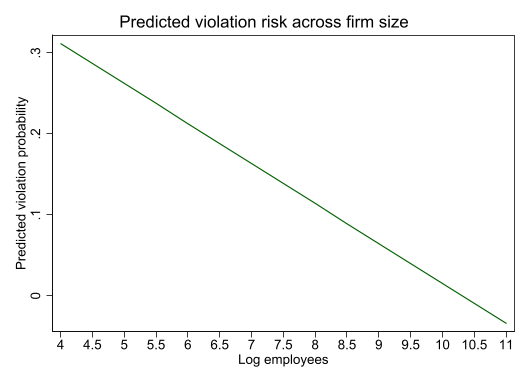
\includegraphics[width=0.70\textwidth]{../图片/paper_u_shape_size.png}
\caption{员工规模与违规风险的非线性预测}
\label{fig:ushape}
\end{figure}

\section{准实验检验}
仅依赖固定效应回归仍不足以完全解决识别问题。为此，本文根据企业在 2016--2019 年形成的平均技能投入与平均组织规模，构造预处理分组，并考察在 2020 年后共同外部冲击背景下，不同预处理组织能力企业的违规风险演化差异。核心直觉在于，如果组织能力确实具有治理价值，那么在环境更不确定、外部约束更复杂的时期，原本组织能力更强的企业应表现出更好的合规韧性。

表 \ref{tab:did} 的结果支持这一判断。以违规虚拟变量为被解释变量时，高技能预暴露企业在 2020 年后的违规概率相对更低，交互项系数为 $-0.0228$；大规模预暴露企业的系数为 $-0.0521$，且绝对值更大。以违规强度为被解释变量时，对应系数分别为 $-0.0366$ 和 $-0.0811$，结果同样显著。这表明，不仅违规发生概率下降，违规事件累积强度也更低。图 \ref{fig:skilltrend} 和图 \ref{fig:sizetrend} 进一步展示了高低预处理组在时间维度上的差异演化。

\begin{table}[H]
\centering
\caption{准实验检验：预处理组织能力与后冲击合规韧性}
\label{tab:did}
\def\sym#1{\ifmmode^{#1}\else\(^{#1}\)\fi}
\begin{tabular}{l*{4}{c}}
\toprule
                    &\multicolumn{1}{c}{(1)}&\multicolumn{1}{c}{(2)}&\multicolumn{1}{c}{(3)}&\multicolumn{1}{c}{(4)}\\
\midrule
high\_skill\_pre $\times$ post\_2020&     -0.0228\sym{**} &                     &     -0.0366\sym{***}&                     \\
                    &    (0.0094)         &                     &    (0.0124)         &                     \\
\addlinespace
注册资本对数        &      0.0165\sym{***}&      0.0152\sym{**} &      0.0258\sym{***}&      0.0237\sym{***}\\
                    &    (0.0061)         &    (0.0061)         &    (0.0082)         &    (0.0082)         \\
\addlinespace
上市年限            &      0.0103\sym{***}&      0.0128\sym{***}&      0.0213\sym{***}&      0.0251\sym{***}\\
                    &    (0.0016)         &    (0.0016)         &    (0.0020)         &    (0.0021)         \\
\addlinespace
high\_size\_pre $\times$ post\_2020&                     &     -0.0521\sym{***}&                     &     -0.0811\sym{***}\\
                    &                     &    (0.0094)         &                     &    (0.0125)         \\
\addlinespace
Constant            &     -0.3179\sym{***}&     -0.3135\sym{***}&     -0.5623\sym{***}&     -0.5551\sym{***}\\
                    &    (0.1187)         &    (0.1181)         &    (0.1595)         &    (0.1585)         \\
\midrule
Observations        &       28289         &       28289         &       28289         &       28289         \\
R-squared           &       0.007         &       0.008         &       0.016         &       0.018         \\
Treatment           &高技能预暴露         &大规模预暴露         &高技能预暴露         &大规模预暴露         \\
\\
\bottomrule
\end{tabular}
\end{table}

\begin{figure}[H]
\centering
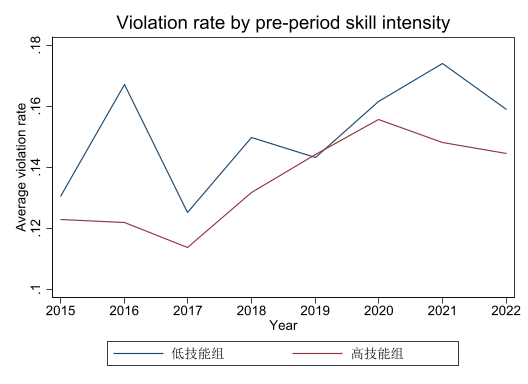
\includegraphics[width=0.72\textwidth]{../图片/paper_skill_trend.png}
\caption{高低技能预暴露企业的违规率趋势}
\label{fig:skilltrend}
\end{figure}

\begin{figure}[H]
\centering
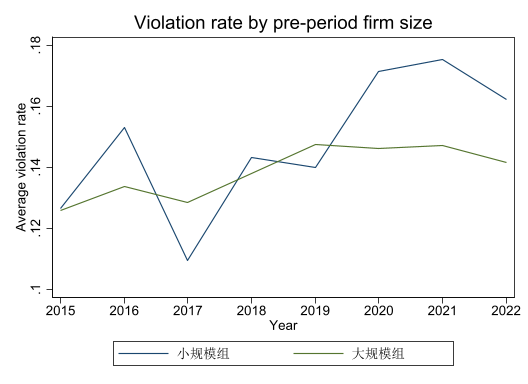
\includegraphics[width=0.72\textwidth]{../图片/paper_size_trend.png}
\caption{高低规模预暴露企业的违规率趋势}
\label{fig:sizetrend}
\end{figure}

需要指出的是，安慰剂检验并不完全支持强平行趋势假设。表 \ref{tab:placebo} 显示，以 2018 年作为虚拟冲击时，预处理分组与假冲击的交互项仍然显著为负。这意味着预处理组织能力较强的企业可能原本就沿着更优的违规轨迹演进。因此，本文将该部分结果解释为“组织能力提升合规韧性的有力证据”，但不将其表述为严格的因果识别结论。

\begin{table}[H]
\centering
\caption{安慰剂检验}
\label{tab:placebo}
\def\sym#1{\ifmmode^{#1}\else\(^{#1}\)\fi}
\begin{tabular}{l*{2}{c}}
\toprule
                    &\multicolumn{1}{c}{(1)}&\multicolumn{1}{c}{(2)}\\
\midrule
high\_skill\_pre $\times$ placebo\_2018&     -0.0228\sym{**} &                     \\
                    &    (0.0100)         &                     \\
\addlinespace
注册资本对数        &      0.0170\sym{***}&      0.0156\sym{**} \\
                    &    (0.0061)         &    (0.0061)         \\
\addlinespace
上市年限            &      0.0103\sym{***}&      0.0130\sym{***}\\
                    &    (0.0016)         &    (0.0017)         \\
\addlinespace
high\_size\_pre $\times$ placebo\_2018&                     &     -0.0531\sym{***}\\
                    &                     &    (0.0100)         \\
\addlinespace
Constant            &     -0.3270\sym{***}&     -0.3246\sym{***}\\
                    &    (0.1191)         &    (0.1181)         \\
\midrule
Observations        &       28289         &       28289         \\
R-squared           &       0.007         &       0.008         \\
Placebo treatment   &高技能预暴露         &大规模预暴露         \\
\\
\bottomrule
\end{tabular}
\end{table}

\section{机制分析}
主结果虽然表明组织能力与违规风险之间存在稳健的负向联系，但如果不能进一步说明作用通道，这一结论仍然停留在 reduced-form 层面。基于组织经济学视角，本文认为组织能力影响违规风险的关键，不在于企业是否抽象地“更规范”，而在于企业能否形成足够细密的执行网络，将规则约束嵌入业务流程与日常决策之中。为此，本文聚焦两个互补但并不等价的机制变量：一是以行政员工对数衡量的\textbf{行政执行网络}，二是以业务员工对数衡量的\textbf{业务执行网络}。前者更接近制度落实、文档记录和内部管理层级，后者更接近前台执行、流程衔接和业务覆盖。

机制检验分为两个步骤。第一步检验组织规模和技能员工规模是否显著推动执行网络扩张。第二步将执行网络变量纳入违规回归，以考察组织能力的主效应是否通过这些中介变量被部分吸收。这样的设计虽然不能完全等同于严格意义上的结构中介分析，但足以用于识别组织能力在何种具体维度上与更低的违规风险更为一致。

表 \ref{tab:mech} 第 (1) 和第 (2) 列显示，组织规模和技能员工规模均显著促进行政执行网络与业务执行网络扩张。具体来看，技能员工规模对数对行政执行网络和业务执行网络的系数分别为 0.1957 和 0.2145，均在 1\% 水平上显著；组织规模对数的系数分别为 0.3175 和 0.3632，也同样高度显著。这意味着组织能力提升并不是一个单一维度的变化，而是系统性地改变了企业内部的岗位配置与执行架构。从经济含义上看，这说明高技能员工扩张往往伴随着更多的业务支撑岗位与协调岗位，从而提高企业吸收复杂监管要求和执行内部控制的能力。

第 (3) 列进一步将行政执行网络与业务执行网络同时纳入违规方程。结果显示，业务执行网络的系数为 $-0.0141$，在 1\% 水平上显著，而行政执行网络的系数不显著；与此同时，员工规模和技能员工规模的负向系数仍然存在，但绝对值有所收缩。这个结果非常关键。它表明，组织能力降低违规风险，并不是通过简单增加管理层级或行政岗位来实现，而更可能依赖于业务流程本身的执行密度、协同能力和记录能力。换言之，真正有助于降低违规风险的，不是“更多管理”，而是“更强执行”。

第 (4) 列进一步引入滞后机制变量，以减弱业务执行网络与违规风险之间的同步性偏误。结果显示，滞后业务执行网络仍表现出边际负向作用，系数为 $-0.0064$，在 10\% 水平上显著；相反，滞后行政执行网络依然不显著。与主结果中滞后技能员工规模仍显著为负的发现结合起来，可以形成较为一致的解释链条：企业先通过技能型人力资本积累提升组织能力，再通过扩展和强化业务执行网络降低未来违规风险。

从一般性层面看，这一机制证据说明，企业合规能力并不是抽象的“治理质量”或“文化氛围”，而是可以落实为具体的组织结构安排。高质量人力资本之所以重要，并不只是因为其提升了平均教育水平，而是因为它使企业得以建立更为有效的执行网络，进而减少信息遗漏、流程断裂和规则执行偏差。从具体性层面看，本文的机制结果尤其强调业务执行网络的作用，这意味着在中国上市公司场景下，前台业务覆盖、流程衔接和执行链条完整性，可能比单纯增加行政层级更能降低违规风险。图 \ref{fig:mechanism} 也直观展示了这一点：随着技能员工规模上升，业务执行网络明显同步扩张。

\begin{table}[H]
\centering
\caption{机制检验：组织能力、执行网络与违规风险}
\label{tab:mech}
\def\sym#1{\ifmmode^{#1}\else\(^{#1}\)\fi}
\begin{tabular}{l*{4}{c}}
\toprule
                    &\multicolumn{1}{c}{(1)}&\multicolumn{1}{c}{(2)}&\multicolumn{1}{c}{(3)}&\multicolumn{1}{c}{(4)}\\
\midrule
员工规模对数        &      0.3175\sym{***}&      0.3632\sym{***}&     -0.0131\sym{**} &                     \\
                    &    (0.0407)         &    (0.0465)         &    (0.0056)         &                     \\
\addlinespace
技能员工规模对数    &      0.1957\sym{***}&      0.2145\sym{***}&     -0.0095\sym{***}&                     \\
                    &    (0.0261)         &    (0.0280)         &    (0.0034)         &                     \\
\addlinespace
注册资本对数        &      0.0891\sym{***}&      0.0508\sym{**} &      0.0256\sym{***}&      0.0084         \\
                    &    (0.0211)         &    (0.0257)         &    (0.0063)         &    (0.0069)         \\
\addlinespace
上市年限            &      0.0056\sym{*}  &      0.0070\sym{*}  &      0.0100\sym{***}&      0.0070\sym{***}\\
                    &    (0.0030)         &    (0.0041)         &    (0.0014)         &    (0.0016)         \\
\addlinespace
ln\_admin\_emp        &                     &                     &      0.0061         &                     \\
                    &                     &                     &    (0.0046)         &                     \\
\addlinespace
ln\_business\_emp     &                     &                     &     -0.0141\sym{***}&                     \\
                    &                     &                     &    (0.0033)         &                     \\
\addlinespace
L1\_ln\_skill\_emp     &                     &                     &                     &     -0.0092\sym{**} \\
                    &                     &                     &                     &    (0.0038)         \\
\addlinespace
L1\_ln\_admin\_emp     &                     &                     &                     &      0.0070         \\
                    &                     &                     &                     &    (0.0054)         \\
\addlinespace
L1\_ln\_business\_emp  &                     &                     &                     &     -0.0064\sym{*}  \\
                    &                     &                     &                     &    (0.0039)         \\
\addlinespace
Constant            &      0.1419         &     -0.2975         &     -0.3122\sym{***}&     -0.0619         \\
                    &    (0.3663)         &    (0.4735)         &    (0.1200)         &    (0.1340)         \\
\midrule
Observations        &       30675         &       30675         &       30675         &       25954         \\
R-squared           &       0.243         &       0.147         &       0.009         &       0.004         \\
Mechanism           &行政执行网络         &业务执行网络         &通道纳入主回归         &    滞后通道         \\
\\
\bottomrule
\end{tabular}
\end{table}

\begin{figure}[H]
\centering
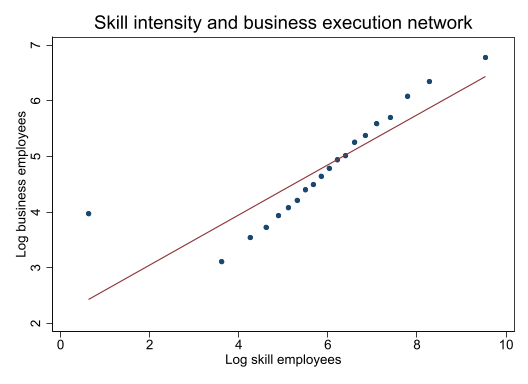
\includegraphics[width=0.72\textwidth]{../图片/paper_mechanism_business.png}
\caption{技能员工规模与业务执行网络}
\label{fig:mechanism}
\end{figure}

\section{结论与启示}
本文基于 2015--2022 年中国上市公司面板数据，系统考察了组织规模、人力资本结构与企业违规风险之间的关系。研究结果表明，在行业和年份固定效应、公司固定效应以及滞后解释变量框架下，组织能力与违规风险之间总体存在显著而稳健的负向联系，其中技能员工规模的作用尤为稳定。进一步地，基于预处理组织能力与 2020 年后共同冲击构造的比较分析显示，预先具有更强技能投入和更大组织规模的企业在后期表现出更高的合规韧性。机制检验则进一步表明，组织能力的治理作用主要通过强化业务执行网络实现，而非依赖单纯的行政扩张。

\subsection*{经济意义}
本文的经济意义主要体现在两个方面。其一，研究将企业违规风险从传统的“外部监管后果”命题，拓展为“组织能力约束下的经济行为结果”命题。换言之，违规并不仅仅由惩罚和监督决定，还受到企业内部执行体系是否成熟的影响。其二，本文揭示了人力资本在公司治理中的一个更具体角色：高技能员工并不仅仅提高企业的平均生产率，更重要的是，它可能帮助企业构建更完整的执行链条和更高质量的流程控制。这使得人力资本投资具有超越生产效率的治理外部性。

\subsection*{研究局限}
尽管本文已经在识别策略和机制检验上做出推进，但研究仍存在若干局限。第一，违规变量按公告年份聚合，无法精确刻画违规真实发生时点。第二，当前样本尚未纳入完整财务报表、股权结构、董事会特征和审计质量等治理变量，因此仍可能存在遗漏变量问题。第三，准实验部分的安慰剂检验未能完全支持强平行趋势假设，这意味着预处理组织能力较强的企业可能本身就具有更优的违规演化路径。第四，行政执行网络和业务执行网络仍是组织结构的代理变量，而非对内部控制制度和执行质量的直接观察。

\subsection*{政策启示}
本文的政策启示并不局限于“加强处罚”这一传统思路。首先，监管部门在推进企业合规建设时，可以更加重视企业内部组织能力，特别是高质量人力资本和业务执行体系的建设。对监管而言，鼓励上市公司提升合规岗位专业化、业务流程可追踪性和信息处理能力，可能比单纯增加披露频率更能从根源上抑制违规。其次，企业自身的治理改革不应只停留在形式上的制度设计，而应把治理资源真正配置到执行网络之中。再次，对于资本市场参与者而言，员工结构和组织能力变量或许可以成为评估企业长期治理质量的重要补充信息。总体而言，若将组织能力视为治理的一部分，则提升企业合规水平的政策工具箱也应从外部惩罚逐步扩展到内部能力建设。

\section*{参考文献}
\begin{enumerate}
\item Baucus, M. S. (1994). Pressure, opportunity and predisposition: A multivariate model of corporate illegality. \textit{Journal of Management}, 20(4), 699--721.
\item Becker, G. S. (1968). Crime and punishment: An economic approach. \textit{Journal of Political Economy}, 76(2), 169--217.
\item Dyck, A., Morse, A., \& Zingales, L. (2010). Who blows the whistle on corporate fraud? \textit{The Journal of Finance}, 65(6), 2213--2253.
\item Fama, E. F., \& Jensen, M. C. (1983). Separation of ownership and control. \textit{Journal of Law and Economics}, 26(2), 301--325.
\item Jensen, M. C., \& Meckling, W. H. (1976). Theory of the firm: Managerial behavior, agency costs and ownership structure. \textit{Journal of Financial Economics}, 3(4), 305--360.
\item Shleifer, A., \& Vishny, R. W. (1997). A survey of corporate governance. \textit{The Journal of Finance}, 52(2), 737--783.
\end{enumerate}

\end{document}
